\chapter{相关原理分析}
\label{xiangguanyuanli}
在本章中,将针对本文涉及的关键技术的原理进行分析和解读,这些关键技术是指导本文工作开展的理论支撑,只有把这些技术原理充分理解后,才能解决设计过程中遇到的难题,才能进行一系列的优化工作。这些技术原理包括,图像表示原理,SIFT算法原理,spark内存技术原理,spark任务调度原理,spark 性能优化原理以及HDFS存储原理。
\section{图像表示原理}
在计算机中,图像的数字表达形式其实是一个二维矩阵,矩阵中的每个数值就是我们常说的图像的像素点。在现实生活中,我们看到的图像大多数是彩色的,在这种情况下,图像数字化表达时,一个像素点值就包含了三个分量,分别是R,G,B,这个三个分量的取值为0到255,三个分量的不同取值和混搭,就构成了我们现实生活中看到的所有色彩。但是在图像处理中,灰度图像更为常见,因为除了色彩信息之外,灰度图像中包含了所有彩色图片包含的信息,不会有任何的区别,包括像形状特征,纹理特征等等,但是灰度图像需要的保存空间比彩色图像的空间更小,因为在灰度图像表示中,像素点只包含一个分量,所以大大缩小了保存的空间以及提升了读写的速率。本文的设计工作就是建立在灰度图像之后,我们将原始的图片都进行了灰度化处理,后续的所有处理都在此基础上进行。

灰度图像的每个像素用一个字节保存,对RGB图像进行灰度化,是对图像中RGB三个分量进行加权平均得到最终的灰度值,加权公式~\ref{jiaquan}所示:
\begin{equation}\label{jiaquan}
 Gray = 0.11B + 0.59G + 0.3R
\end{equation}

理解好基础的图像原理,是Spark下图像基础库SparkImgLib实现的理论指导,因为SparkImgLib包含了在Spark下图像的表示以及一些基础处理接口。
\section{SIFT算法原理}
\label{sec:sift}
在本小节中,将会对SIFT算法进行详细分析,它是Spark下特征提取系统的最核心算法。

在如上一章的介绍,SIFT算法一个提取局部特征的算法,它通过构建物体尺度空间,在尺度空间中去搜索满足要求的特征点,这些特征点是具有很大抵抗物理噪声能力的,比如旋转噪声,光照噪声,遮挡噪声等,这些点在Lower论文中是被称为具有尺度不变性的特征点。它的基本特点如下:
\begin{itemize}
\item 局部不变性好,在物体受到比较严重的物理噪声干扰下,依然可以准确的描述出物体原有的特性。
\item 特征信息丰富,一个特征点是采用长度为128的一维向量进行表示。
\item 可扩展性强,可以很方便的与其他形式的特征向量进行联合。
\end{itemize}

SIFT算法大体可以划分为5个步骤,分别是高斯塔建立,高斯差分塔建立,极点检测,消除边缘响应,关键点方向的分配和描述,接下来,将会对这几个步骤进行分析:
\begin{compactenum}
\item 高斯塔建立\\SIFT算法中的尺度空间的具体表示就是图像的高斯金字塔(gaussian pyramid),从\ref{fig:gausspy}图就可以看出来,为什么图像的尺度空间被称为gaussian pyramid,同一张图片的不同尺寸,从小到大,依次往下排列,形成了塔状。建立gaussian pyramid时,先将一张进行高斯模糊及尺寸放大,得到其以下面一层的图片,然后再在新的图片的基础上继续做高斯模糊及尺寸放大。具体的层数是算法的一个参数,SIFT论文中一组金字塔的高度是7层。当一组gaussian pyramid被建立后,抽取倒数第三层的图片作为下一组gaussian pyramid的顶层图片,依次得到后面所有组数的gaussian pyramid,同样组数也是SIFT 算法中的一个参数,Lower论文中组数大小为8组。一组高斯金字塔如图~\ref{fig:gausspy} 所示:
\begin{figure}[htp]
\centering
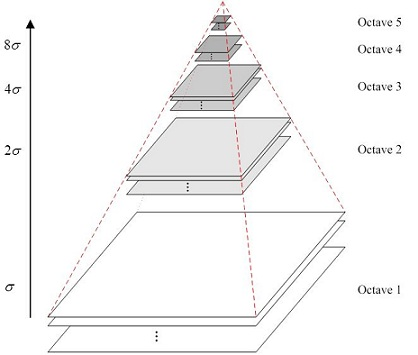
\includegraphics{gausspy}
\caption{图像的一组高斯金字塔}
\label{fig:gausspy}
\end{figure}

上面在介绍gaussian pyramid时,提到了尺度空间(scale-space),scale space是SIFT算法中一个非常重要的概念。scale space最早是由Iijima\upcite{Iijima}于1962年提出的,后经witkin\upcite{Witkin}和Koenderink\upcite{Koenderink} 等人的推广逐渐得到关注,在计算机视觉邻域使用广泛。它的基本思想是,使用一个尺度参数,然后得到物体在不同的尺度参数下一段图像序列,最后在获取的序列上进行斑点检测或者是轮廓提取。尺度空间形象的比喻就像物体在人的视线中有近到远的消失。尺度理论的数学表达式如公式~\ref{chidu} 所示,公式中,高斯模板的维度使用m和n表示,图像的像素位置使用x和y表示,尺度空间因子使用$\delta$表示。
\begin{equation}\label{chidu}
L(x,y,\delta)=G(x,y,\delta)*I(x,y)
\end{equation}

其中,*表示卷积运算,G(x,y,$\delta$)为高斯函数,
\begin{equation}\label{gauss}
G(x,y,\delta)=\frac{1}{2\pi{\delta}^2}e^{-\frac{(x-m/2)^2+(y-n/2)^2}{2\delta^2}}
\end{equation}

\item 高斯差分金字塔建立\\如果将gaussian pyramid中上下相邻的两张图片做减操作,即将两张图片的像素值相减,那么就可以得到高斯差分金子塔(DOG),SIFT算法中,极点的检测实际上是在DOG的基础上进行的,目的在于减少检测的运算量。 DOG如图~\ref{fig:gaussDog} 所示:
\begin{figure}[htp]
\centering
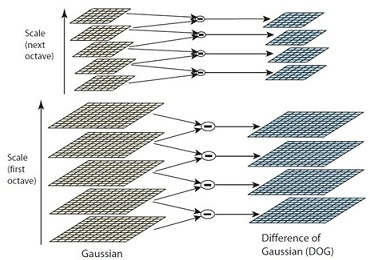
\includegraphics{gaussDog}
\caption{高斯差分金子塔}
\label{fig:gaussDog}
\end{figure}

这里更加仔细的解释一下为什么使用高斯差分金子塔并不会影响提取结果的正确性,在图像中最稳定的特征对应着尺度归一化的高斯拉普拉斯(简称gauss-laplace)函数${\delta}^2{\nabla}^2{G}$的极值。而高斯差分函数(gauss-difference)与尺度归一化的高斯拉普拉斯函数${\delta}^2{\nabla}^2{G}$存在等式关系,关系推到如下:
\begin{equation}\label{dog_1}
\frac{\partial{x}}{\partial{\delta}}=\delta\nabla^2G
\end{equation}

利用差分近似代替微分,则有:
\begin{equation}\label{dog_2}
\delta\nabla^2G=\frac{\partial{x}}{\partial{\delta}}\approx\frac{G(x,y,k\delta)-G(x,y,\delta)}{k\delta-\delta}
\end{equation}

因此就有:
\begin{equation}\label{dog_3}
G(x,y,k\delta)-G(x,y,\delta)\approx(k-1)\delta^2\nabla^2G
\end{equation}

从上面的公式推导,我们就可以看出高斯拉普拉斯函数和高斯差分函数是常数关系,两者极值关系如图~\ref{fig:py_dog}所示,最下方的曲线为DOG函数,上方为高斯拉普拉斯算子:
\begin{figure}[htp]
\centering
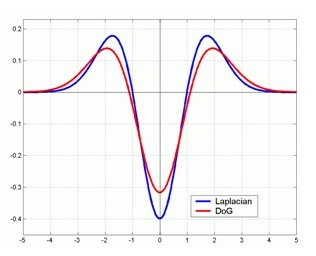
\includegraphics{py_dog}
\caption{gauss-laplace和gauss-difference极值关系比较}
\label{fig:py_dog}
\end{figure}

因此,我们就可以使用gauss-difference替代gauss-laplace进行图像特征点检测,公式如下所示:
\begin{equation}\label{dog_detect}
D(x,y,\delta)=\Bigl(G(x,y,k\delta)-G(x,y,\delta)\Bigr)*I(x,y)=L(x,y,k\delta)-L(x,y,\delta)
\end{equation}

\item 极点检测\\因为SIFT中的特征点是从高斯差分金字塔上的极值中得到的(这里先强调一下,不是所有的极值点都是特征点,后续会有专门的步骤将一些噪声大的极点删除点),因此需要在guass-difference上对极值的判断,这里的判断是指将需要判断是否为极值的像素点和它为同一层像素点的相邻的8个点以及上下两层共18(9*2)点进行比较,看是否是所有比较点的极大点还是极小点。具体如图~\ref{fig:pole_detect} 所示:
\begin{figure}[htp]
\centering
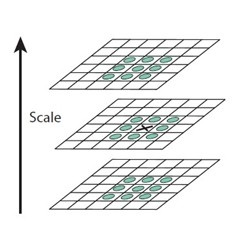
\includegraphics{pole_detect}
\caption{高斯差分图像上的极点检测}
\label{fig:pole_detect}
\end{figure}

\item 关键点精确定位\\在上一点中,本文强调了,不是所有在高斯差分金字塔上检测到的极值点都是关键点,因为整个检测过程是在一个离散空间上进行的,因此检测出来的极值点不是严格的极值点,图~\ref{fig:keypoint_detect}解释了为什么检测出来的极值点不是严格的极点。在这种情况下,就需要对获取到的极值曲线进行子像素插值 (Sub-pixel Interpolation),目的在于获取更加严格的极值点,以保证特征点的质量。在进行插值操作完成后,为了使所有关键点表现的更加平滑,因为如果两个相邻的关键点的差值很大,会造成比较大的噪声,这样的特征点效果不好。因此在SIFT 算法中还会对关键点进行拟合,拟合具体表现就是对高斯差分函数进行Taylor展开式,拟合后的函数如~\ref{Tayor}所示。根据拟合后的guassin-different函数,就可以设置一些阈值进行判断,去掉一些不满足要求的特征点,使得提取的特征点更加稳定。
\begin{figure}[htp]
\centering
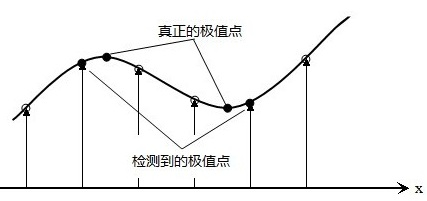
\includegraphics{keypoint_detect}
\caption{检测出来的极点和严格意义上的极点比较}
\label{fig:keypoint_detect}
\end{figure}


\begin{equation}\label{Tayor}
D(X)=D+\frac{\partial{D}^T}{\partial{X}}X+\frac{1}{2}X^T\frac{\partial^2{D}}{\partial{X}^2}X
\end{equation}

\item 关键点方向分配和描述\\当图像的所有关键点被检测出来后,接下来就要为关键点分配一个主方向,主方向的确定首先要统计关键点以邻域内的所有关键点的梯度的模值和方向,计算公式如\ref{mozhi}所示,其中关键点的尺度空间值表示为L,然后将以上得到的梯度按方向的进行归类(这里的类别共有36种,从0到360度,每10度为1类,比如,10度,20度,30度,...,360度),统计每一类中总模值的大小,最大的模值的方向就为主方向,同时也会选取总模值大于主方向的模值的80\%为辅方向,辅方向的建立是为了增强关键点的鲁棒性。上述过程最终会形成一个直方图,具体如图\ref{fig:direct_histogram}所示。
\begin{equation}\label{mozhi}
m(x,y)=\sqrt{L(x+1,y)-{L(x-1,y)}^2+L(x,y+1)-{L(x,y-1)}^2}
\end{equation}
\begin{equation}\label{fangxiang}
\theta(x,y)=\tan^{-1}\Bigl({\frac{L(x,y+1)-L(x,y-1)}{L(x+1,y-L(x-1,y)}}\Bigr)
\end{equation}
\end{compactenum}

\begin{figure}[htp]
\centering
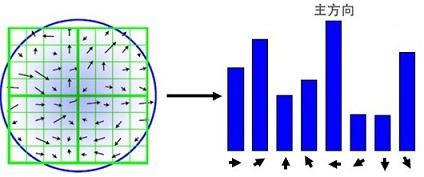
\includegraphics{direct_histogram}
\caption{关键点方向直方图}
\label{fig:direct_histogram}
\end{figure}

在关键点的主方向被确认后,SIFT算法还没有结束,因为计算机处理的只有数字信息,因此必须采用严格数字符号将关键的信息描述出来,SIFT算法中采用长度为128的一维向量对一个关键点进行描述,向量的含义为以关键点为中心,4*4 窗口区域内(每个窗口为一个关键点),计算所有关键点在8个方向上的梯度,共计128个梯度信息。至此,SIFT特征描述向量生成完毕。

在上述5个步骤中,构建高斯金字塔和极点检测是最为耗时的两个。构建高斯金字塔时需要对每张图片进行高斯滤波,高斯滤波是一个时间复杂度为O(N3) 的操作,这里的N与图像大小成正比。图~\ref{fig:gausspy}中仅显示了一组金字塔,而SIFT算法往往需要构建多组金字塔,使得构建高斯金字塔的时间复杂度达到O(O*I*N3),其中O为高斯塔的组数,I为高斯塔的层数。极点检测则是在整个金字塔组上进行的,相当于在一个维度为4的空间(组,层,长,宽)中搜索极值点,它的时间复杂度为O(O*I*N2)。SIFT算法流程中既包含高斯滤波和图像缩放等通用性较强的操作,也含有构建高斯(查分)金字塔、极点检测、消除边缘响应等通用性较差的操作。它的空间复杂度和时间复杂度都比较高,当有海量的图片需要进行特征提取时,占用内存较多,所需的处理时间也会很长。这也是我们使用Spark去加速SIFT算法的原因。

只有充分理解SIFT算法原理之后,才能比较好的在Spark上实现大规模特征提取工作。

\section{Spark核心技术原理}
在这一小节中,将会对Spark中三个核心技术原理进行分析,它们分别是内存编程原理,任务调度原理,性能优化。这三个技术在本文的设计起非常重要的地位,只有将这些技术理解透彻后,才能自如的解决开发过程中遇到的问题。
\subsection{Spark内存编程原理}
Spark区别于其他的大数据处理框架,比如Hadoop\upcite{Hadoop},在于它是一个内存计算的大数据处理框架,它可以将处理的中间结果保存在内存中,后续的计算可以在此基础上直接运行,提升了执行的效率。那么,这么多的数据保存在内存中,这就必须基于分布式内存的数据结构抽象,让开发人员基于该数据结构进行操作,只要操作这些数据,它们就是位于集群的内存中的。上面说的内存抽象数据结构就是RDD(Resilient Distributed Dataset),RDD是Spark最核心的概念,接下来将从RDD的底层实现原理,RDD的操作类型,RDD的缓存原理,RDD 的依赖关系和DAG的生成这几方面分析RDD。
\subsubsection{RDD的底层实现原理}
RDD的基本单元是分区(Partition),一个RDD由多个分区组成,每个分区都会被逻辑映射成一个Block,一个Block会被一个Task执行,这些Block由BlockManager管理,BlockManager负责管理这些Block在集群内的分布。整个过程如图~\ref{fig:blockmanager}所示:
\begin{figure}[htp]
\centering
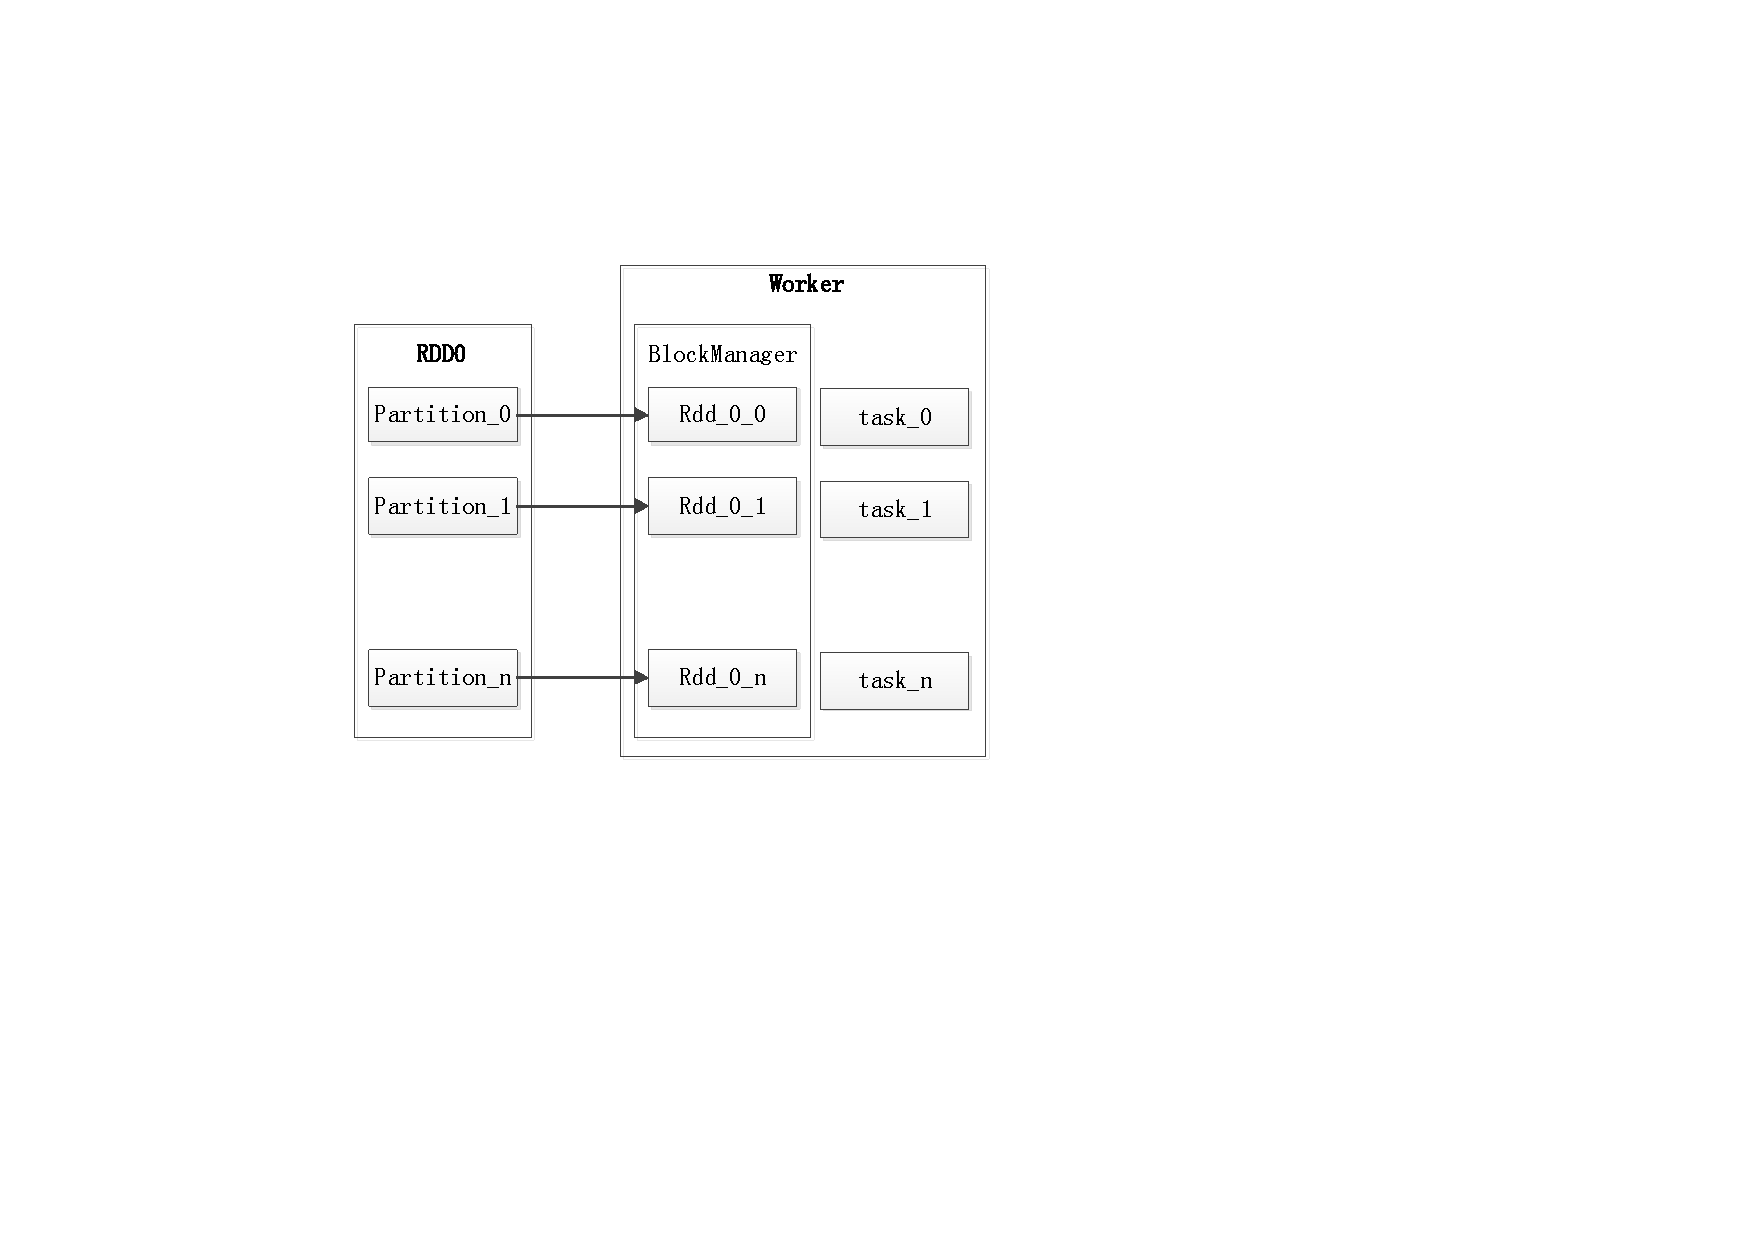
\includegraphics{blockmanager}
\caption{RDD Partition的存储和计算模型}
\label{fig:blockmanager}
\end{figure}

\subsubsection{RDD的操作类型}
RDD提供的操作可以分为两种类型,分别是transformtion(转换)和action(动作),表\ref{tab:trans}和表\ref{tab:action}分别列出了常用的转换操作和动作操作。所有transformation类型的算子被调用时,Spark不会马上进行算子的执行,Spark会使用一个有向图(DAG)将这些操作记录下来,当一个action算子被调用时,那么在这之前的所有transformation操作全都被执行。这种设计会让Spark 运行得更加高效率,因为可能在动作操作时,被操作的数据集会变得比较小。
\begin{table}[h] %开始一个表格environment,表格的位置是h,here。
\caption{RDD转换操作} %显示表格的标题
\centering
\label{tab:trans}
\begin{tabular}{p{6cm}|p{8cm}} %设置了每一列的宽度,强制转换。
\hline
\hline
转换  & 含义 \\ %用&来分隔单元格的内容 \\表示进入下一行
\hline %画一个横线,下面的就都是一样了,这里一共有4行内容
map(func)  & 对所有分区上的数据都执行func操作\\
\hline
filter(func)  & 具有数据过滤的功能,对所有分区上的数据使用func条件进行过滤\\
\hline
flatMap(func)  & 这个函数和map是具有同样功能,区别在于它处理完后会将结果变成一个一维数组\\
\hline
mapPartitions(func) & 类型于map,但是独立在RDD的每一个分片上运行,因此func的类型必须是Iterator[T]=>Iterator[U]\\
\hline
mapPartitionWithSplit(func) & 类似于mapPartitions,但是func带有一个整型参数表示分片的索引值,func的函数类型为(Int,Iterator[T])=>Iterator[U]\\
\hline
sample(withReplacement,fraction,seed) & 根据fraction指定比例对数据进行采用\\
\hline
distinct(numTasks) &对分区上的数据进行去重操作\\
\hline
\hline
\end{tabular}
\end{table}

\begin{table}[h] %开始一个表格environment,表格的位置是h,here。
\caption{RDD动作操作} %显示表格的标题
\centering
\label{tab:action}
\begin{tabular}{p{6cm}|p{8cm}} %设置了每一列的宽度,强制转换。
\hline
\hline
动作  & 含义 \\ %用&来分隔单元格的内容 \\表示进入下一行
\hline %画一个横线,下面的就都是一样了,这里一共有4行内容
reduce(func)  & 通过函数func聚集数据集中的所有元素\\
\hline
collect()  & 将所有的分区的运算结果收集到Driver上\\
\hline
count()  & 返回数据集的个数\\
\hline
first() & 返回数据集的第一个元素\\
\hline
take(n) & 这个算法和collect有所区别,collect是返回所有结果,take是返回前n个结果\\
\hline
takeSample(withReplacement,num,seed) & 在所有分区的数据上进行采用\\
\hline
saveAsTextFile(path) & 将运算结果以文本的方式保存到HDFS中\\
\hline
saveAsSequenceFile(path) & 将运算结果以序列化的方式保存到HDFS中\\
\hline
countByKey() 根据key信息统计记录的条数\\
\hline
\hline
\end{tabular}
\end{table}

\subsubsection{RDD的缓存原理}
RDD的特点在于它是一个内存数据结构,所有对它的操作是在内存中完成的,这也是为什么Spark在迭代次数多的任务中计算的速率要远快于Hadoop。在Spark中,某个数据集会被后续操作使得到,或者是整体使用的频率十分高,这时候就可以将其缓存到内存中,即持久化一个数据集在内存中。具体可以通过persist()或cache()方法可以标识一个要被持久化的RDD。persist()和cache()的实现如下:
\begin{lstlisting}[language=Java,numbers=none,frame=none]
/**Persist this RDD with the default storage level('MEMORY_ONLY').*/
def persist(): this.type = persist(StorageLevel.MEMORY_ONLY)
/**Persist this RDD with the default storage level('MEMORY_ONLY').*/
def cache(): this.type = persist()
\end{lstlisting}

假设首先进行了RDD0$\rightarrow$RDD1$\rightarrow$RDD2的计算作业,如果RDD1已经被缓存在内存中,那么后续在进行RDD0$\rightarrow$RDD1$\rightarrow$RDD3的计算作业时,就不需要从头开始,直接从RDD1往下执行作业即可,因此计算速度得到了很大的提升,具体过程如下图\ref{fig:rdd_cache}所示:
\begin{figure}[htp]
\centering
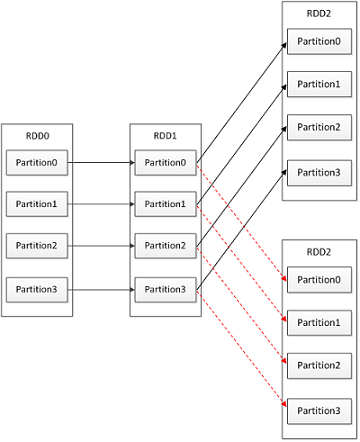
\includegraphics{rdd_cache}
\caption{RDD 缓存加速原理}
\label{fig:rdd_cache}
\end{figure}

缓存的rdd有可能会丢失,或者因为内存不足而删除,但是rdd有完整的容错机制,保证在rdd丢失或者删除的情况下计算依然可以正确执行。
\subsubsection{RDD的依赖关系和DAG的生成}
一个Spark应用中,不同的RDD间存在依赖关系,依赖关系分为窄依赖(narrow dependency)和宽依赖(wide dependency),窄依赖和宽依赖的定义如下:
\begin{itemize}
\item 窄依赖,窄依赖是指父RDD的分区结果和子分区使用是一个1对1的关系,如图\ref{fig:dependency}左边部分显示
\item 宽依赖,宽依赖是指父RDD的分区结果和子分区使用是一个多对1的关系,如图\ref{fig:dependency}右边部分显示
\end{itemize}
\begin{figure}[htp]
\centering
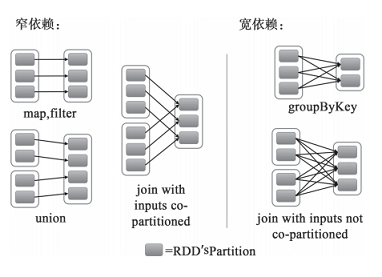
\includegraphics{dependency}
\caption{RDD窄依赖和宽依赖对比}
\label{fig:dependency}
\end{figure}
在Spark应用开发中,RDD会经过很多转换操作,每个转换操作都会生成一个新的RDD,这些转换操作最后会形成一个有向图(Directed Acyclic Graph,简称DAG)。这个DAG记录着RDD间的依赖关系,借助这些依赖关系,能保证一个RDD被计算前,所有它所依赖的parent RDD都已经完成了计算。Spark会根据DAG对算子进行stage的划分,划分的依据是,rdd间是窄依赖关系的划分到一个stage中,rdd间是宽依赖的划分到不同的stage 中。一个stage 中的task可以并行执行,不同stage的task则要顺行执行。
\subsection{Spark任务调度原理}
Spark任务调度框架主要由三个模块支撑起,它们分别是DAGScheduler,SchedulerBackend及TaskScheduler。首先DAGScheduler分析用户提交的应用,根据依赖关系建立DAG,然后将DAG 划分为不同的Stage,而stage中包含所要执行的tasks。SchedulerBackend负责整个集群交互,收集可用的资源信息,然后将这些信息上报TaskScheduler。TaskScheduler将从SchedulerBackend获取到的资源信息以及从DAGScheduler生成的tasks进行一个资源的分配,将tasks分配的合适的资源上面。整个流程如图\ref{fig:schedulerfw}所示:
\begin{figure}[htp]
\centering
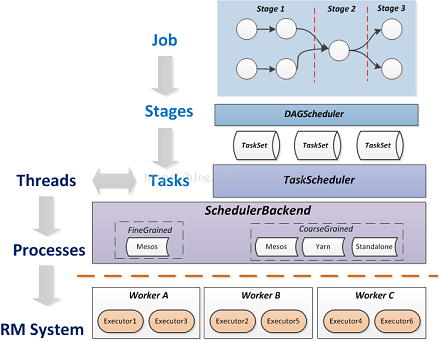
\includegraphics{schedulerfw}
\caption{Spark任务调度框架}
\label{fig:schedulerfw}
\end{figure}
\subsubsection{DAGScheduler}
DAGScheduler的功能是对应用程序提交的task根据依赖关系进行stage的划分,将窄依赖关系的task划分到一个stage中,然后将task一个集合的形式进行打包,形成taskset,再将taskset传递给TaskScheduler。
\subsubsection{SchedulerBackend}
SchedulerBackend负责和整个集群打交道,收集集群的资源信息,并且将这些信息上报给TaskScheduler。SchedulerBackend中有两种调度方式,分别是粗粒度和细粒度两种,运行时具体是哪一种取决于集群的运行模式。粗粒度下,tasks是按照Executor进行分配的,而在细粒度下,task是按照线程进行分配的。
\subsubsection{TaskScheduler}
TaskScheduler的任务是负责将从DAGScheduler传递上来的Tasks分配到合适的工作节点上面,对于Taks的分配策略有两种,分别是FIFO(先进先出)以及FIFA(公平调度)。TaskScheduler中存在两个列表,一个是可以被launch的tasks列表,另外的是可以被use的worker列表,TaskScheduler如同一个管家,按照列表的顺序,吩咐相应worker去处理相应的tasks。但是如果一直按照这种方式,可能是某个worker或者是某几个worker会经常处于忙碌状态(因为他们都比其他work的计算能力强,一直在"抢"任务),而大部分worker一直处理闲状态。所以为了避免这种情况,TaskScheduler会对Worker进行shuffle操作,任意挑选worker放在worker列表的前面。

\subsection{Spark性能优化原理}
在本小节中,将介绍Spark的性能优化原理,因为Spark是处理大数据的框架,因此性能优化是非常有必要的。接下来将从几个方面分析spark的性能问题
\subsubsection{调度和分区优化}
在Spark中,一个分区是对应着一个task的,即一个分区是一个并行的单元,那么是不是分区的数量越多,一个Spark应用就会运行的越快呢?其实并不是这样,不是分区数越多,运行的速度的越快,因为当分区数量十分大时,task的调用开销也会变得很大,有可能出现tasks的调度时间比任务运行的总时间还要长。所以,在制定分区数量时要综合考虑集群系统的资源和被处理作业的数据量。

在分区优化问题中,还有一个倾斜(skew)的问题。倾斜可以分为数据倾斜和任务倾斜,两者存在关系,数据倾斜会引发任务倾斜。
\begin{compactenum}
\item 数据倾斜\\数据倾斜是指数据被划分的不均匀,一个task被分配了很多的处理数据,有可能比所有task分配的还要多,在这种情况下就会导致负载的不均衡,下面是一些常见的引发Spark在出现数据倾斜的原因:
\begin{itemize}
\item key数据分布不均匀,因为spark中默认是按照Hash方式进行分区,如果某个key的数据特别多,就会造成分到某个key上的数据特别多,最后造成某个分区的数据特别多,也就出现了数据倾斜。
\item 结构化数据表设计问题
\item 某些SQL语句产生数据倾斜
\end{itemize}

\item 任务倾斜\\产生任务倾斜的原因较为隐蔽,有可能是服务器架构的原因,有可能是JVM的原因,有可能是线程池的原因,也有可能是业务本省的原因。比如在本文设计中就发现,即使是两个任务的处理数据的总大小一样,但是仍然会产生任务倾斜,这和处理问题的具体场景有关系,在SIFT算法中,算法的时间复杂度和图片的尺寸大小有关系的。
\end{compactenum}

\subsubsection{内存存储优化}
因为spark是内存计算的大数据处理框架,因此内存存储优化也是十分重要的内容。内存调优过程中,有三个方向值得考虑,分别是JVM调优,OOM问题调优及磁盘临时目录空间优化。
\begin{compactenum}
\item JVM调优\\不同的JAVA对象都有一个对象头,这些信息有时候比数据本身的信息还要大,比如只有一个Int属性的对象。还有一些链式结构,它们会包含一些指针信息。因此在开发的过程要选好数据类型和数据结构,尽量减少一些链式结构的使用;减少对象的嵌套;可以考虑使用数字ID或者是枚举对象,而不是字符串作为key的关键数据。
\item OMM问题调优\\在spark开发过程中,内存溢出(OutOfMemoryError)是一个经常会遇到的问题,发生内存溢出的原因是Java虚拟机创建的对象太多,在进行垃圾回收时,虚拟机分配的堆空间已经用满了,与heap space有关。解决这类问题有两种思路,一种是减少App的内存占用空间消耗,另一种是增大内存资源的供应。具体设计时,可以查看程序中是否有循环创建对象的地方,程序中应该减少这种代码的存在,或者可以调整JVM中的Xmx(最大堆)和Xms(最小堆)参数的大小。另外,还要查看在做shuffle类操作符时是否创建的Hash表过大,在这种情况下,可以通过增加任务数,即分区数来提升并行度,减少每个任务的输入数据,减少内存占用来解决问题。
\end{compactenum}

\subsubsection{磁盘临时目录空间优化}
Spark在进行shuffle的过程中,中间结果会写到spark在磁盘的临时目录中,如果临时目录过小的话,会造成No Space left on device异常,在这种情况下可以配置多个盘块来扩展Spark的磁盘临时目录,让更多的数据可以写到磁盘,加快I/O速度。
\subsubsection{网络传输优化}
Spark是大数据处理框架,因此集群中数据传输也是影响应用性能的重要因素。如果可以减少数据传输的次数或者是传输的大小,可能会极大的提高应用的性能。下面将分析spark中数据传输优化的场景。
\begin{compactenum}
\item 大局部变量的传输\\在spark的分布式处理算子中,如果使用了不是算子内部的变量,那么Spark会为每个task生成一个这样的变量,那么如果这个变量十分大,比如是一个大数组,而且执行的任务又特别多,那么网络的传输耗费就会特别大。下面就是一个例子的展示,其中factor 就是一个变量,它在map 任务中被使用:
\begin{lstlisting}[language=Java,numbers=none,frame=none]
val factor = 3
rdd.map(num => num*factor)
\end{lstlisting}

面对这种情况,我们可以采用Spark中Broadcast或者是共享变量这两种方式来解决大外部变量传输的问题,通过这两种方式,Spark只会为Worker生成需要的外部变量,而不是为每个task生成一个外部变量,减少了局部变量的传输开销。
\item 大结果收集\\在spark的开发中,会经常用到collect操作,collect操作将各个分区的结果收集到一个数组,返回到driver。如图\ref{fig:collect}如果收集的结果过大,就会拖慢应用的执行时间,甚至造成内存溢出。
\begin{figure}[htp]
\centering
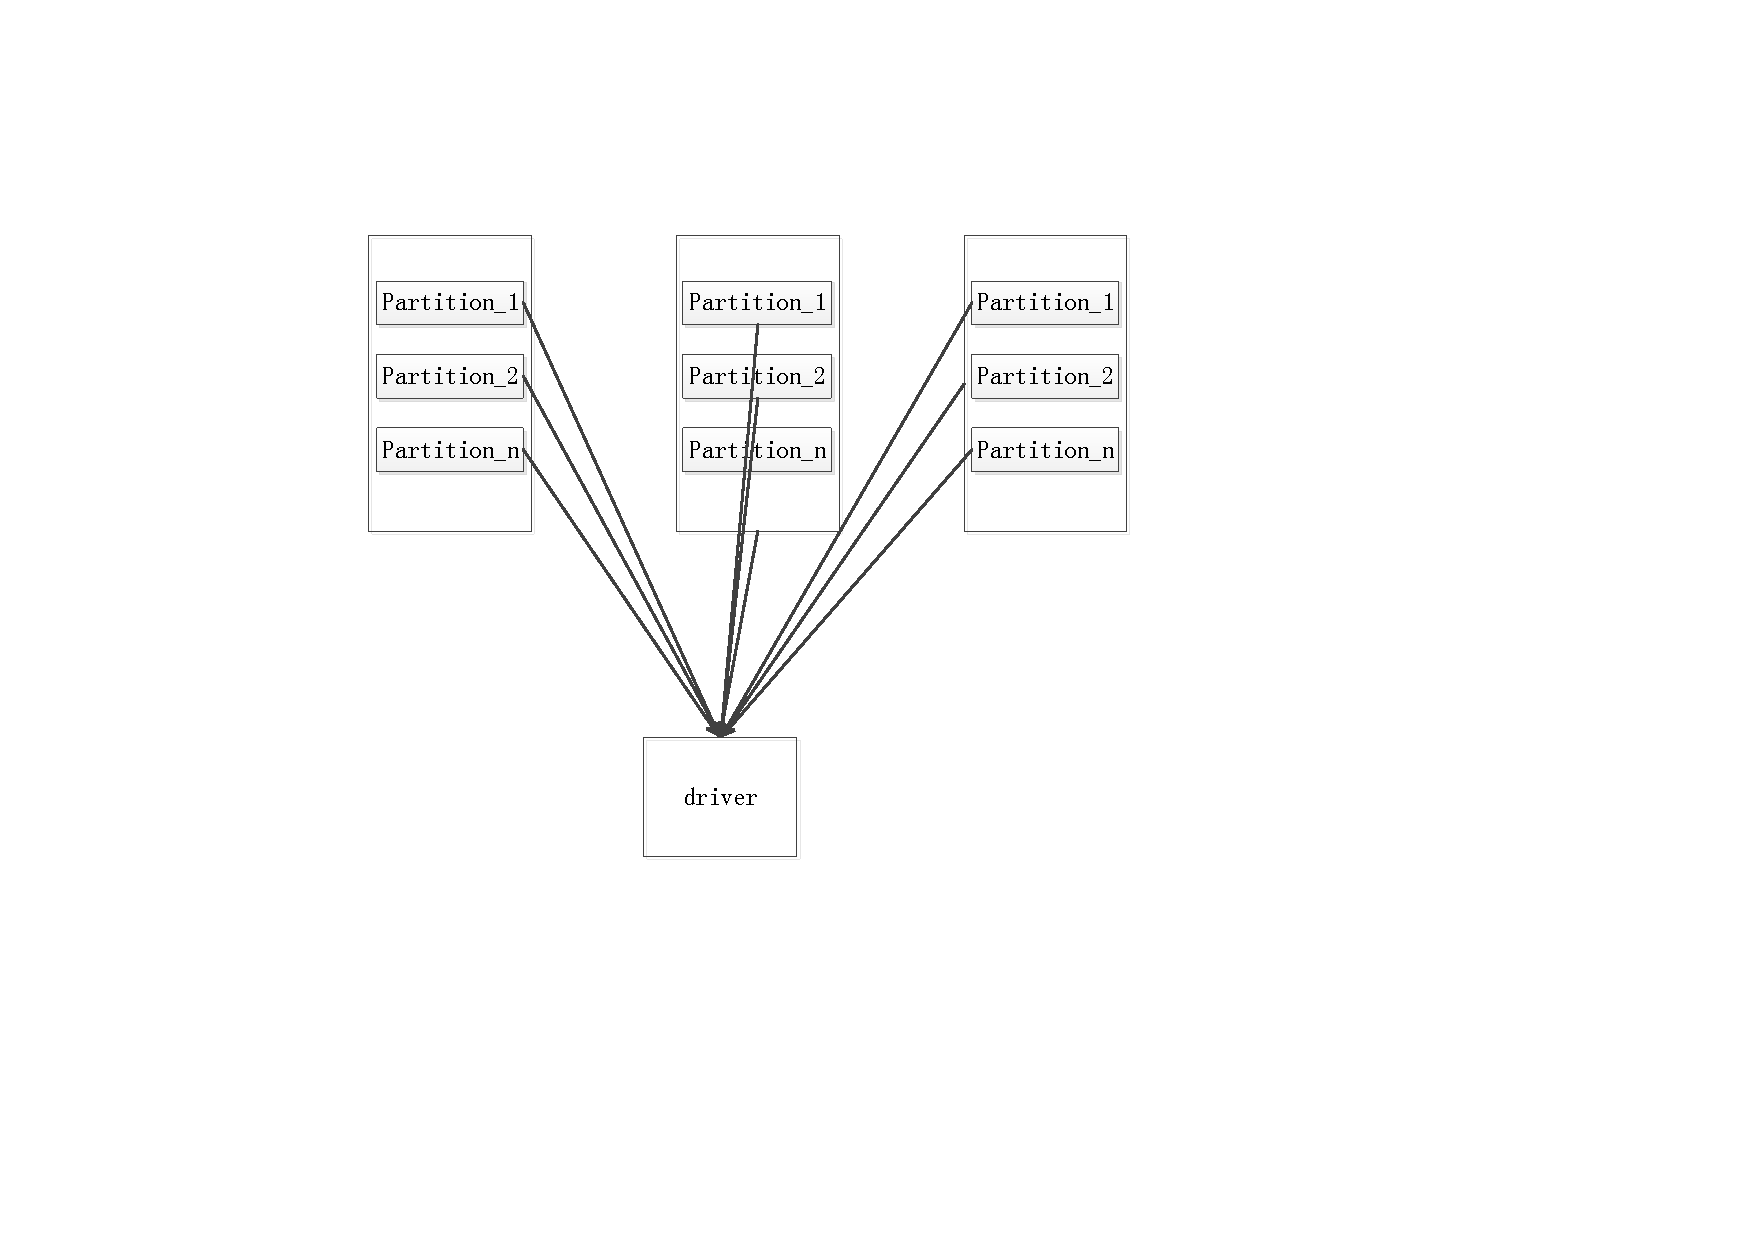
\includegraphics{collect}
\caption{collect操作收集所有分区}
\label{fig:collect}
\end{figure}
面对这种情况,如果收集的结果过大,可以将数据分布式的存储在HDFS或者其他的分布式持久化层上,这样可以减少单机数据的I/O开销和单机内存的存储压力。
%%\subsubsection{序列化与压缩}
\end{compactenum}
\section{分布式存储原理}
在大数据处理场景下,需要的处理的数据集往往是很大的,比如100T,那么使用单节点的存储方案是基本不可能的,无论是数据的存储空间或者是数据的安全方面,单节点是无法适用需求的。因此,需要一种集群式的的存储方案来应对大数据的场景下的数据保存,HDFS分布式文件是根据google的三大论文中的The google fileSystem文章开发出来的。HDFS是一个Master-Slave的架构,里面有Namenode,DataNode及SecondaryNameNode三种角色,NameNode负责管理数据的元数据信息,DataNode负责数据的data数据的保存,SecondaryNameNode负责数据的备份。HDFS是按照Block为单位进行数据存储的,在HDFS中一个Block的大小通常为64M,从这里就可以看出HDFS 中的Block的大小比我们Linxu的文件系统的Block要大很多,这也是为了在大数据场景下提升数据的读写效率。在写入数据的时候,如果被写入文件如果大于64M,HDFS会进行数据的划分,按照块的大小进行划分,那么一个文件就可能被划分为几个块,进行分布式存储。同样在读取数据的时,hdfs客户端将文件名以及字节的偏移发送给NameNode,NameNode根据字节偏移量转化成Block偏移,然后将给偏移量返回客户端,客户端根据该偏移量信息到DataNode上进行数据的读取,后续的操作也不需要经过NameNode。
\section{GPU特征提取原理}
因为在实验数据比较上,我们和GPU下的特征提取进行了比较,因此,在这小节中的介绍GPU的相关原理。GPU最开始的时候是应用在图像显示领域的,作为显卡使用,后面因为其出色的并行加速能力,逐渐应用于科学计算,机器学习及深度学习的领域中。我们通过是将CPU上相关需要加速的算法改写成GPU 版本,是程序中可以并行的代码区域,在GPU上以多线程方式并行执行,大大提升了程序的运行时间。GPU之所以能够比CPU拥有如此大的并行加速能力,原因在GPU上的计算单元远远多于CPU上的计算单元,GPU上的计算单元可以划分为三个维度,分别设计Grids,Blocks以及Threads,大量的Threads组成一个Block,然后大量的Blocks组成一个Grids,最后由大量的Grids组成强大的计算能力。
\section{本章小结}
本章分析了本文工作的一些技术原理,首先分析SIFT算法原理,主要针对SIFT算法的5个主要步骤进行分析,分析5个步骤的数学原理及在SIFT算法中的作用,然后讨论了SIFT算法的中最为耗时的步骤。在介绍完SIFT算法原理之后,本章节对Spark-SIFT的大数据模块进行原理分析,首先分析了park-SIFT的计算引擎Spark 主要分析Spark核心技术原理,包括Spark的内存编程原理,任务调度原理,性能优化原理。接着又分析了了充当Spark-SIFT 系统存储层的HDFS 文件系统的一些核心原理。最后,介绍了作为本文设计工作对比的GPU特征提取的一些基本原理。


